\documentclass[12pt,a4paper,twoside]{report}
\usepackage[a4paper,outer=1cm,inner=3cm,top=2cm,bottom=1cm]{geometry}
\usepackage{setspace}
\usepackage{polyglossia}
\usepackage{fontspec}
\usepackage{xltxtra}
\usepackage{listings}
\usepackage{titlesec}
\usepackage{color}
\usepackage{xcolor}

\defaultfontfeatures{Scale=MatchLowercase}
\setsansfont[Mapping=tex-text]{Helvetica}
\renewcommand*{\familydefault}{\sfdefault}

\usepackage{amsmath}
\usepackage{amsfonts}

\titleformat{\section}{\normalfont\fontsize{25}{25}\bfseries\centering}{\thesection}{1em}{}
\newcommand{\sectionbreak}{\clearpage}

\title{
	Компьютерный праткикум по\\
	линейной алгебре.\\
	Расчётное задание №1\\[4em]
	\large {
		Тема: Матрицы и операции над ними.\\
		Обратная матрица. Системы векторов.\\
		Линейная зависимость и независимость.\\
		Системы линейных уравнений. \\
		Метод Гаусса. Ранг и база системы векторов.\\[4em]
	}
}
\author{Вилков Кирилл Олегович, группа 14ПИ}
\date{05.10.14}

\makeatletter
\def\Title{Расчётное задание №1}
\let\theauthor\@author
\makeatother

\usepackage{fancyhdr}
\pagestyle{fancy}
\fancyhf{}
\fancyhead[LE,RO]{\thepage}
\fancyhead[RE,LO]{\Title \qquad \theauthor}
\fancyheadoffset{0mm}
\fancyfootoffset{0mm}
\setlength{\headheight}{15pt}
\renewcommand{\headrulewidth}{1pt}
\renewcommand{\footrulewidth}{0pt}

\usepackage{tocloft}

\setcounter{tocdepth}{1}
\setcounter{secnumdepth}{0}
\renewcommand\contentsname{Содержание}
\tocloftpagestyle{fancy}

\usepackage{listings}
%\usepackage{courier}

\definecolor{dkgreen}{rgb}{0,0.6,0}
\definecolor{gray}{rgb}{0.5,0.5,0.5}
\definecolor{mauve}{rgb}{0.58,0,0.82}

\lstset{
	frame=tb,
	xleftmargin=20pt,
	language=Matlab,
	aboveskip=3mm,
	belowskip=3mm,
	showstringspaces=false,
	columns=flexible,
	basicstyle={\small\ttfamily},
	numbers=none,
	breaklines=true,
	breakatwhitespace=true
	tabsize=2
}

\newcommand{\showcode}[1]{
	%\begin{minipage}{\linewidth}
		\lstinputlisting{#1}
	%\end{minipage}
}
\newcommand{\showscreen}[1]{
\\ \includegraphics[scale=0.6]{#1} \\
}


\begin{document}

	\maketitle
	\pagestyle{fancy}
	\setcounter{page}{1}
	\tableofcontents
	\newpage

	\renewcommand*{\arraystretch}{1.5}

	\section{Задача 1.24}
\subsection{Задание:}
Решить
$
	\left|
		\begin{matrix}
			2 & x & 6 \\
			3 & 3 & 9 \\
			7 & 4 & 11
		\end{matrix}
	\right|
	= 0
$
\subsection{Решение:}
$
	3 \cdot 11 \cdot x + 2 \cdot 4 \cdot 9 + 2 \cdot 3 \cdot 11 -
	6 \cdot 3 \cdot 4 - 6 \cdot 3 \cdot 7 - 7 \cdot 9 \cdot x = 0
	\\[1ex]
	-30x - 60 = 0
	\\[1ex]
	x = -\dfrac{60}{30} = 2
$
\subsection{Проверим результат в среде Wolfram Mathematica:}
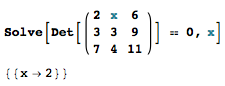
\includegraphics[scale=0.6]{task/1_24/screen.png}
\subsection{Ответ:}
Компьютерная проверка подтвердила полученный результат.

	\section{Задача 1.25}
\subsection{Задание:}
Найти матрицу обратную к
$
	A =
	\begin{pmatrix}
		2 & 4 & 0 & 1 \\
		3 & -3 & 5 & 0 \\
		-1 & 0 & 1 & 1 \\
		2 & 1 & 1 & 0 \\
	\end{pmatrix}
$
\; методом алгебраических дополненй.
\subsection{Решение:}
Найдём $ \det A $ чтобы убедиться что $ \exists A^{-1} $:
\\[1em]
$
	\det A =
	\begin{vmatrix}
		2 & 4 & 0 & 1 \\
		3 & -3 & 5 & 0 \\
		-1 & 0 & 1 & 1 \\
		2 & 1 & 1 & 0 \\
	\end{vmatrix}
	=
	\begin{vmatrix}
		3 & 4 & -1 & 0 \\
		3 & -3 & 5 & 0 \\
		-1 & 0 & 1 & 1 \\
		2 & 1 & 1 & 0 \\
	\end{vmatrix}
	=
	\begin{vmatrix}
		3 & 4 & -1 & 0 \\
		3 & -3 & 5 & 0 \\
		-1 & 0 & 1 & 1 \\
		2 & 1 & 1 & 0 \\
	\end{vmatrix}
	=
	-
	\begin{vmatrix}
		3 & 4 & -1 \\
		3 & -3 & 5 \\
		2 & 1 & 1 \\
	\end{vmatrix}
	=
	5
$
\\[1em]
$ \det A \neq 0 \Rightarrow \exists A^{-1} = \dfrac{D^T}{\det A} $
\\[1em]
$
	d_{11} =
	\begin{vmatrix}
		-3 & 5 & 0 \\
		0 & 1 & 1 \\
		1 & 1 & 0 \\
	\end{vmatrix}
	=
	\begin{vmatrix}
		-3 & 5 & 0 \\
		0 & 1 & 1 \\
		1 & 1 & 0 \\
	\end{vmatrix}
	=
	-
	\begin{vmatrix}
		-3 & 5 \\
		1 & 1 \\
	\end{vmatrix}
	= 8
\\[1em]
	d_{12} =
	\begin{vmatrix}
		3 & 5 & 0 \\
		-1 & 1 & 1 \\
		2 & 1 & 0 \\
	\end{vmatrix}
	=
	-
	\begin{vmatrix}
		3 & 5 \\
		2 & 1 \\
	\end{vmatrix}
	=
	7
\\[1em]
	d_{13} =
	\begin{vmatrix}
		3 & -3 & 0 \\
		-1 & 0 & 1 \\
		2 & 1 & 0 \\
	\end{vmatrix}
	=
	-
	\begin{vmatrix}
		3 & -3 \\
		2 & 1 \\
	\end{vmatrix}
	=
	-9
\\[1em]
	d_{14} =
	\begin{vmatrix}
		3 & -3 & 5 \\
		-1 & 0 & 1 \\
		2 & 1 & 1 \\
	\end{vmatrix}
	=
	\begin{vmatrix}
		-3 & 5 \\
		1 & 1 \\
	\end{vmatrix}
	-
	\begin{vmatrix}
		3 & -3 \\
		2 & 1 \\
	\end{vmatrix}
	=
	-8 - 9 = -17
\\[1em]
	d_{21} =
	\begin{vmatrix}
		4 & 0 & 1 \\
		0 & 1 & 1 \\
		1 & 1 & 0 \\
	\end{vmatrix}
	=
	4
	\begin{vmatrix}
		1 & 1 \\
		1 & 0
	\end{vmatrix}
	+
	\begin{vmatrix}
		0 & 1 \\
		1 & 1
	\end{vmatrix}
	= -4 - 1 = -5
\\[1em]
	d_{22} =
	\begin{vmatrix}
		2  & 0 & 1 \\
		-1 & 1 & 1 \\
		2 & 1 & 0 \\
	\end{vmatrix}
	=
	2
	\begin{vmatrix}
		1 & 1 \\
		1 & 0 \\
	\end{vmatrix}
	+
	\begin{vmatrix}
		-1 & 1 \\
		2 & 1 \\
	\end{vmatrix}
	= -2 - 3 = -5
\\[1em]
$

	\section{Задача 1.27}
\subsection{Задание:}
Не вычисляя определитель
$
	\begin{vmatrix}
		2 & 1 & 7 & 8 & 1 \\
		3 & 9 & 7 & 7 & 4 \\
		6 & 5 & 3 & 4 & 3 \\
		8 & 0 & 4 & 9 & 5 \\
		7 & 2 & 9 & 1 & 9 \\
	\end{vmatrix}
$
доказать что он делится нацело на 947.
\subsection{Решение:}
По свойству определителя к любомоу столбцу можно прибавить линейную комбинацию других, и определитель не изменится.
Прибавим к последнему столбцу линейную комбинацию других:
\\
$
	\tilde a_{\bullet 5} =
	10000 \cdot a_{\bullet 1} +
	1000  \cdot a_{\bullet 2} +
	100   \cdot a_{\bullet 3} +
	10    \cdot a_{\bullet 4}
	+ a_{\bullet 5}
$
\\
Тогда определитель принимает вид:
\\[1em]
$
	\begin{vmatrix}
		2 & 1 & 7 & 8 & 21781 \\
		3 & 9 & 7 & 7 & 39774 \\
		6 & 5 & 3 & 4 & 65343 \\
		8 & 0 & 4 & 9 & 80495 \\
		7 & 2 & 9 & 1 & 72919 \\
	\end{vmatrix}
	=
	947 \cdot
	\begin{vmatrix}
		2 & 1 & 7 & 8 & 23 \\
		3 & 9 & 7 & 7 & 42 \\
		6 & 5 & 3 & 4 & 69 \\
		8 & 0 & 4 & 9 & 85 \\
		7 & 2 & 9 & 1 & 77 \\
	\end{vmatrix}
$
\\[1em]
Значит определитель делится нацело на 947
\subsection{Компьютерная проверка в среде Wolfram Mathematica:}
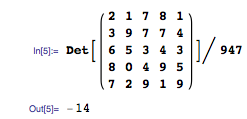
\includegraphics[scale=0.6]{task/1_27/screen1.png}
\subsection{Вывод:}
Компьютерная проверка показала что определитель действительно делится нацело на 947.

	\section{Задача 1.31}
\subsection{Задание:}
Вычислить
$
	\begin{vmatrix}
		1 & 2 & 3 & \cdots & n - 1 & n \\
		-1 & 0 & 3 & \cdots & n - 1 &  n \\
		-1 & -2 & 0 & \cdots & n - 1 & n \\
		\vdots & \vdots & \vdots & \ddots & \vdots & \vdots \\
		-1 & -2 & -3 & \cdots & -(n - 1) & 0 \\
	\end{vmatrix}
$.
\subsection{Решение:}
Вынесем общий множитель из каждого столбца определителя (вынесем из каждого столбца номер этого столбца),
тогда определитель принимает вид:
\\[1em]
$
	n! \cdot
	\begin{vmatrix}
		1 & 1 & 1 & \cdots & 1 & 1 \\
		-1 & 0 & 1 & \cdots & 1 &  1 \\
		-1 & -1 & 0 & \cdots & 1 & 1 \\
		\vdots & \vdots & \vdots & \ddots & \vdots & \vdots \\
		-1 & -1 & -1 & \cdots & -1 & 0 \\
	\end{vmatrix}
$
\\[1em]
Докажем методом мат. индукции что
$
	\begin{vmatrix}
		1 & 1 & 1 & \cdots & 1 & 1 \\
		-1 & 0 & 1 & \cdots & 1 &  1 \\
		-1 & -1 & 0 & \cdots & 1 & 1 \\
		\vdots & \vdots & \vdots & \ddots & \vdots & \vdots \\
		-1 & -1 & -1 & \cdots & -1 & 0 \\
	\end{vmatrix}
	= 1
$
\\[1em]
Проверим базу $ n = 1 $: $ |1| = 1 $
\\
Предположим что утверждение верно для $ n $, тогда докажем для $ n + 1 $:
\\[1em]
$
	\begin{vmatrix}
		1 & 1 & 1 & \cdots & 1 & 1 \\
		-1 & 0 & 1 & \cdots & 1 &  1 \\
		-1 & -1 & 0 & \cdots & 1 & 1 \\
		\vdots & \vdots & \vdots & \ddots & \vdots & \vdots \\
		-1 & -1 & -1 & \cdots & -1 & 0 \\
	\end{vmatrix}_{n + 1}
	=
	\begin{vmatrix}
		1 & 1 & 1 & \cdots & 1 & 1 \\
		-1 & 0 & 1 & \cdots & 1 &  1 \\
		-1 & -1 & 0 & \cdots & 1 & 1 \\
		\vdots & \vdots & \vdots & \ddots & \vdots & \vdots \\
		0 & 0 & 0 & \cdots & 0 & 1 \\
	\end{vmatrix}_{n + 1}
	=
	1 \cdot
	\begin{vmatrix}
		1 & 1 & 1 & \cdots & 1 & 1 \\
		-1 & 0 & 1 & \cdots & 1 &  1 \\
		-1 & -1 & 0 & \cdots & 1 & 1 \\
		\vdots & \vdots & \vdots & \ddots & \vdots & \vdots \\
		-1 & -1 & -1 & \cdots & -1 & 0 \\
	\end{vmatrix}_{n}
$
\\[1em]
Утверждение доказано.
\\[1em]
Получается что
$
	\begin{vmatrix}
		1 & 2 & 3 & \cdots & n - 1 & n \\
		-1 & 0 & 3 & \cdots & n - 1 &  n \\
		-1 & -2 & 0 & \cdots & n - 1 & n \\
		\vdots & \vdots & \vdots & \ddots & \vdots & \vdots \\
		-1 & -2 & -3 & \cdots & -(n - 1) & 0 \\
	\end{vmatrix}
	=
	n!
$
\subsection{Компьютерная проверка:}
Выполним проверку в среде Wolfram Mathematica при $ n = 8 $:
\\
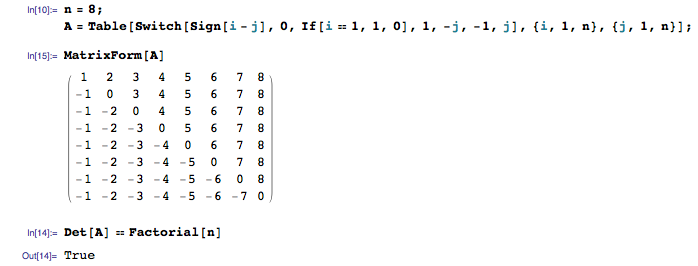
\includegraphics[scale=0.6]{task/1_31/screen1.png}
\subsection{Вывод:}
Компьютерная проверка подтвертила правильность полученной формулы.

	%\section{Задача 1.33}
\subsection{Задание:}
Вычислить:
\\[1em]
$
	\begin{vmatrix}
		0 & 1 & 1 & 1 & \cdots & 1 & 1 \\
		1 & a_1 & 0 & 0 & \cdots & 0 & 0 \\
		1 & 0 & a_2 & 0 & \cdots & 0 & 0 \\
		\vdots & \vdots & \vdots & \vdots & \ddots & \vdots & \vdots \\
		1 & 0 & 0 & 0 & \cdots & a_{n-1} & 0 \\
		1 & 0 & 0 & 0 & \cdots & 0 & a_n \\
	\end{vmatrix}
$
\subsection{Решение:}
Можно заметить что для различных $ n $ определитель такой матрицы равен
$ |A| = -\sum \limits_{i=1}^n \dfrac{1}{a_i} \prod \limits_{i=1}^n a_i $
\\
Докажем методом математической индукции:
\\
При $ n = 2 $:
\\
$
	\begin{vmatrix}
		0 & 1 & 1 \\
		1 & a_1 & 0 \\
		1 & 0 & a_2 &
	\end{vmatrix}
	= -a_1 - a_2
$
\\
Если утверждение верно при $ n $, тогда при $ n + 1 $
\\
$
\begin{vmatrix}
	0 & 1 & 1 & 1 & \cdots & 1 & 1 \\
	1 & a_1 & 0 & 0 & \cdots & 0 & 0 \\
	1 & 0 & a_2 & 0 & \cdots & 0 & 0 \\
	\vdots & \vdots & \vdots & \vdots & \ddots & \vdots & \vdots \\
	1 & 0 & 0 & 0 & \cdots & a_{n} & 0 \\
	1 & 0 & 0 & 0 & \cdots & 0 & a_{n+1} \\
\end{vmatrix}
= (-1)^{n+2} \cdot (-1)^{n+1} \cdot
\begin{vmatrix}
	0 & 1 & 1 & 1 & \cdots & 1 & 1 \\
	1 & a_1 & 0 & 0 & \cdots & 0 & 0 \\
	1 & 0 & a_2 & 0 & \cdots & 0 & 0 \\
	\vdots & \vdots & \vdots & \vdots & \ddots & \vdots & \vdots \\
	1 & 0 & 0 & 0 & \cdots & a_{n-1} & 0 \\
	1 & 0 & 0 & 0 & \cdots & 0 & a_n \\
\end{vmatrix}
- \sum \limits_{i=1}^n \dfrac{1}{a_i} \prod \limits_{i=1}^{n+1} a_i =
- \sum \limits_{i=1}^{n+1} \dfrac{1}{a_i} \prod \limits_{i=1}^{n+1} a_i
$
\subsection{Выполним компьютерную проверку в среде Wolfram Mathematica:}
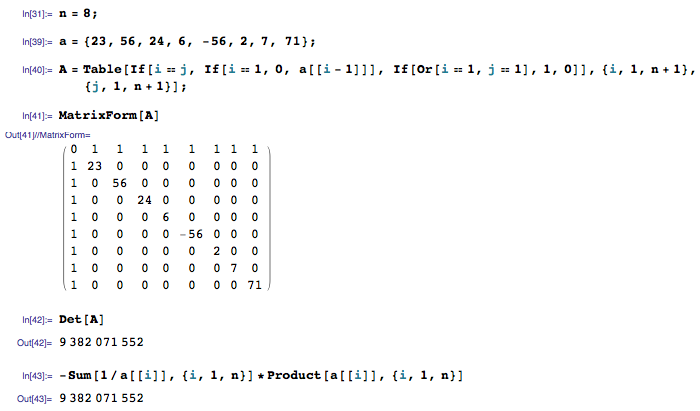
\includegraphics[scale=0.6]{task/1_33/screen.png}
\subsection{Вывод:}
Мы выполнили компьютерную проверку и убедились в верности предположения.

	\section{Задача 1.35}
\subsection{Задание:}
Вычислить $ \det A, A = \{ a_{ij} \} |, i = \overline{1,n}, j = \overline{1,n}, a_{ij} = \min (i,j) $
\subsection{Решение:}
Докажем методом мат. индукции что $ \det A = 1 $:
\\
Проверим базу индукции: $ |1| = 1 $
\\
Допустим что утверждение верно для $ n $, тогда докажем что оно будет верно для $ n + 1 $:
\\[1em]
$
	\begin{vmatrix}
		     1 &      1 & \cdots &      1 &       1 \\
		\vdots & \vdots & \ddots & \vdots &  \vdots \\
		     1 &      2 & \cdots &      n &       n \\
		     1 &      2 & \cdots &      n &   n + 1 \\
	\end{vmatrix}_{n + 1}
	=
	\begin{vmatrix}
		     1 &      1 & \cdots &      1 &       1 \\
		\vdots & \vdots & \ddots & \vdots &  \vdots \\
		     1 &      2 & \cdots &      n &       n \\
		     0 &      0 & \cdots &      0 &       1 \\
	\end{vmatrix}_{n + 1}
	=
	\begin{vmatrix}
		     1 &      1 & \cdots &      1  \\
		\vdots & \vdots & \ddots & \vdots  \\
		     1 &      2 & \cdots &      n  \\
	\end{vmatrix}_n
$
\\[1em]
В силу мат. индукции предположение доказано.
\subsection{Компьютерная проверка в среде Wolfram Mathematica:}
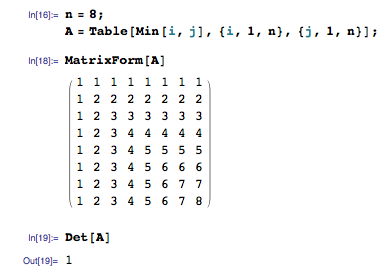
\includegraphics[scale=0.6]{task/1_35/screen1.png}
\subsection{Вывод:}
Компьютерная проверка показала что утверждение верно.


\end{document}
